\documentclass[12pt]{article}

\usepackage[utf8]{inputenc}
\usepackage[T1]{fontenc}
\usepackage[brazil]{babel}

\usepackage{array,latexsym}
\usepackage{amsmath, amsfonts, amssymb, amsthm, mathabx, amstext}
\usepackage{dsfont}
\usepackage{graphicx}

\begin{document}
	\section{Figuras}
		\par Um exemplo deste caso é observado na função de densidade da normal truncada no intervalo $(10,20)$ para as médias $\mu=11$ e $\mu=19$ na Figura \ref{fig_normal}
		\begin{figure}[h!]
			\caption{\label{fig_normal}	Distribuição normal truncada no intervalo $(10,20)$}
			\begin{center}
				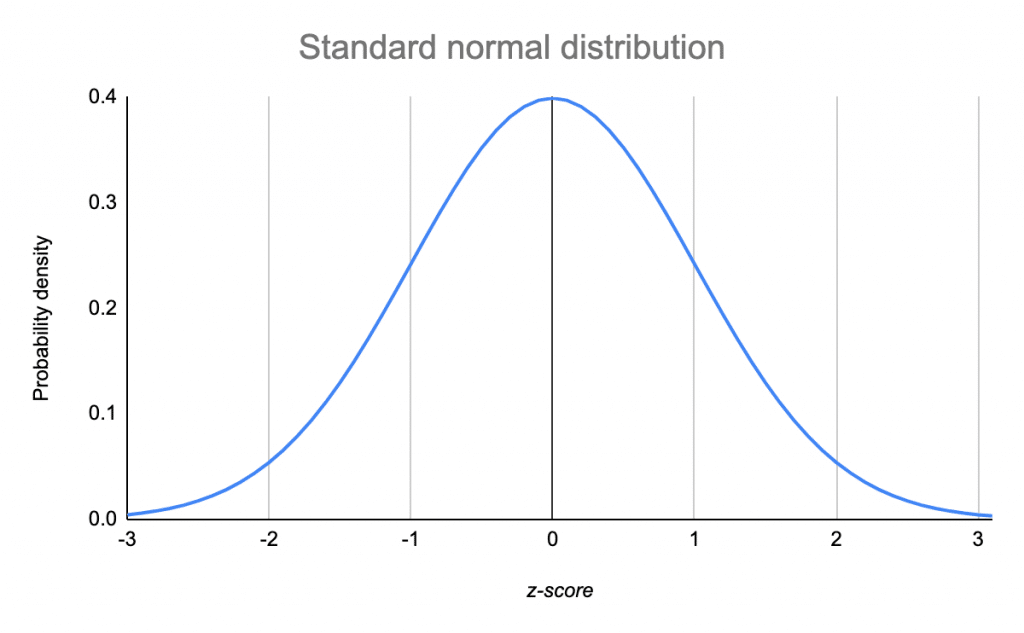
\includegraphics[scale=0.2]{normal}
			\end{center}
		\end{figure}
	
		\par Observe que todas as formas das curvas de densidade da distribuição PERT estão comprimidas dentro do intervalo $(10,20)$ e não cortadas bruscamente como ocorre na distribuição normal truncada na Figura \ref{fig_pert}
		\begin{figure}[h!]
			\caption{\label{fig_pert} Distribuição PERT no intervalo $(10,20)$}
			\begin{center}	
				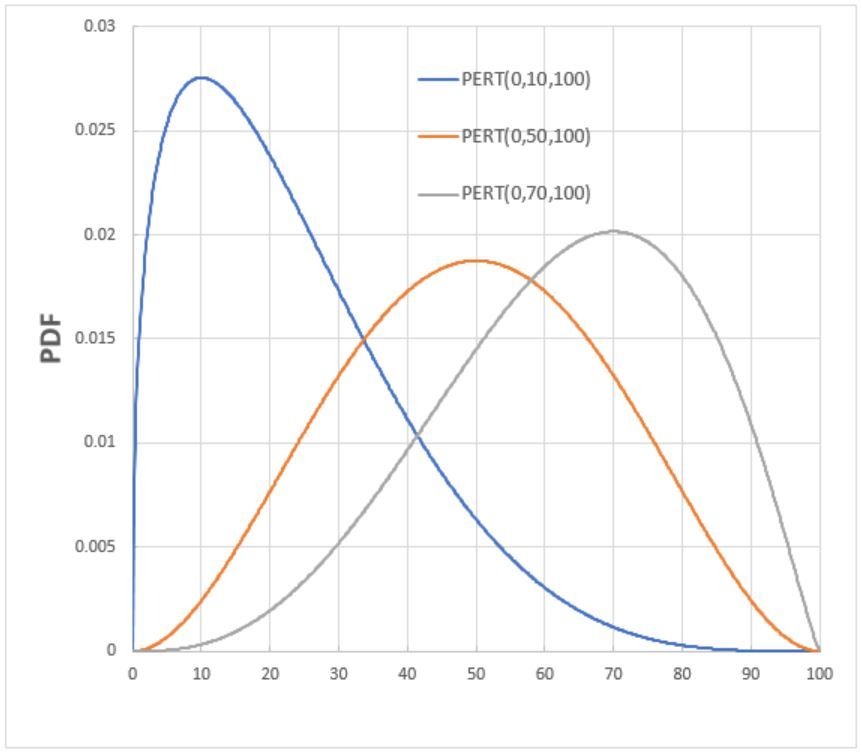
\includegraphics[scale=0.2]{pert}
			\end{center}
		\end{figure}
	
		\begin{figure}[h!]
	 		\centering
	 		\caption{Distribuição PERT novamente}
	 		\label{fig_pert2}
	 		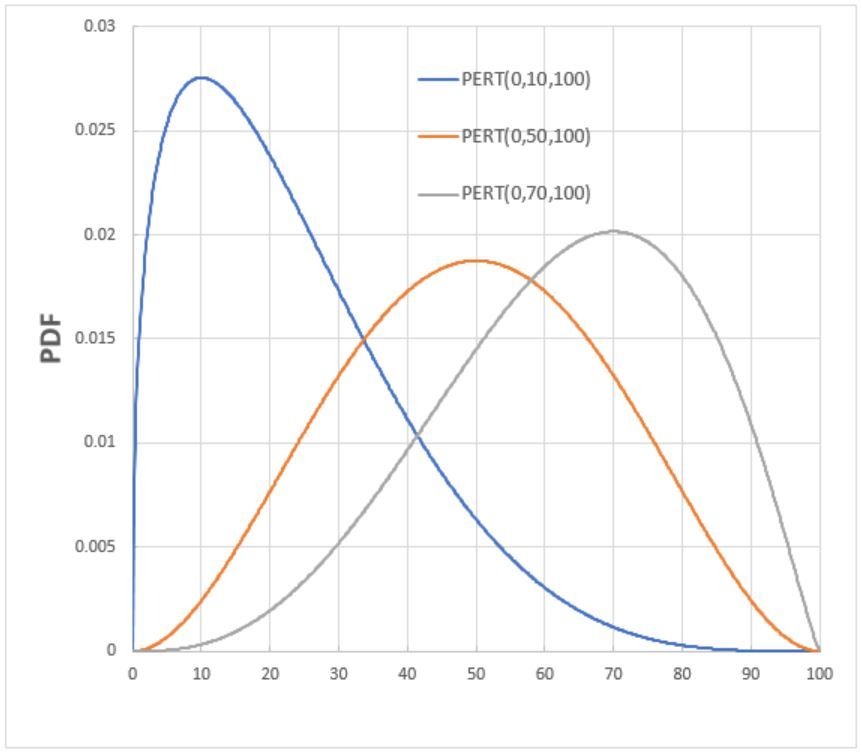
\includegraphics[scale=0.2]{pert}
	 	\end{figure}
	 
	
	
	
\end{document}